%%This is a very basic article template.
%%There is just one section and two subsections.
\documentclass[conference]{IEEEtran}





\usepackage{times}

% *** CITATION PACKAGES ***
%
\usepackage{cite}


% *** GRAPHICS RELATED PACKAGES ***
%
\ifCLASSINFOpdf
  \usepackage[pdftex]{graphicx}

\else

   \usepackage[dvips]{graphicx}

\fi


\usepackage[tight,footnotesize]{subfigure}
%\usepackage[caption=false]{caption}
%\usepackage[font=footnotesize]{subfig}






% *** PDF, URL AND HYPERLINK PACKAGES ***
%
\usepackage{url}
\usepackage[cmex10]{amsmath}


% correct bad hyphenation here
\hyphenation{op-tical net-works semi-conduc-tor Horiz-ontal}
\begin{document}
\title{Arabic Handwriting Recognition using Concavity Features and Classifier Fusion}

%\section{Title}
% author names and affiliations
% use a multiple column layout for up to three different
% affiliations
\author{
\IEEEauthorblockN{Sherif Abdel Azeem}
\IEEEauthorblockA{Electronics Engineering Department\\
American University in Cairo\\
Email: shazeem@aucegypt.edu}
\and
\IEEEauthorblockN{Maha El Meseery}
\IEEEauthorblockA{Electronics Engineering Department \\
American University in Cairo\\
 Email: melmeseery@aucegypt.edu}
%\and
}

% make the title area
\maketitle


\begin{abstract}

This paper presents a simple and  effective technique for the recognition of writer-independent offline handwritten Arabic Digits. The system is based on labeling the white pixels in a   digit's  image into nine different concavity categories. Four different feature vectors are extracted from these labeled concavities. Each feature vector is then introduced to a linear SVM classifiers. The final decision of the system is achieved using classifiers fusion methods. The system has been tested on a database of 10000 Arabic handwritten digits. The presented method achieves a recognition rate of 99.36\% which outperforms all reported results on that Arabic digits database using linear SVM classifier.

\end{abstract}

\IEEEpeerreviewmaketitle

\section{Introduction}

 Handwritten digits recognition has application like office automation, check verification, and postal address reading and sorting. While recognition of handwritten Latin digits has been extensively investigated using various techniques \cite{FE4Liu2003}, too little work has been done on handwritten Arabic digits.

Al-Omari et al. \cite{indiannumerals14} used a scale-, translation-, rotation-invariant feature vector to train a probabilistic neural network (PNN). Their database was composed of 720 digits for training and 480 digits for testing written by 120 persons. They achieved 99.75\% accuracy. Said et al.\cite{EnglishArabic15} used pixel values of the normalized digit images as features. They fed these values to an Artificial Neural Network (ANN). They used a training set of 2400 digits and a testing set of 200 digits written by 20 persons to achieve 94\% accuracy. In \cite{ADBase9}, El-Sherif and Abdelazeem devised a two-stage system for recognizing Arabic digits. The first stage is an ANN fed with a short feature vector to handle easy-to-classify digits. Ambiguous digits are rejected to the more powerful second stage which is an SVM fed with a long feature vector. The system had a good timing performance and achieved 99.15\% accuracy. Note that results of different works cannot be compared because the used databases are not the same. Abdelazeem and El-Sherif \cite{IjdarSherifPaper} conducted a comprehensive study on the problem of Arabic handwritten digits recognition. They reported the performances of different classification methods and several universal feature extraction techniques on the recognition of handwritten Arabic digits. Abdelazeem  \cite{Abdelazeem2009} used several features based on the toplogy of the Arabic digits and achieved 99.25\% recognition rate. %did a comprehensive study on the problem of Arabic handwritten digits recognition. They reported the performances of different classification and universal feature extraction techniques on the recognition of  handwritten Arabic digits. Abdelazeem used several features based on the toplogy of the Arabic digits and achieved 99.25\% recognition rate \cite{Abdelazeem2009}.


There is a wealth of feature extraction techniques in the literature for numeral as well as character recognition in general \cite{TrierFeature}. The input pattern is characterized by a set of N features extracted from the raw data, these features are based on two types of features: statistical and structural. Statistical features such as moment features, transform features, and gradient features are derived from the statistical distribution of the image itself \cite{benchmarking3,Shiagradient}, unlike the structural features such as concavity features , curvature features, geometrical features, and zoning features which are based on the topological and geometerical properties of the digit or character \cite{SirkantangradientContor,visionfeatures5}. Among the various feature extraction techniques, gradient features in particular have proved to be somewhat superior to other feature sets  \cite{benchmarking3,liunormalizegradient}. The  problem with statistical features is that they do not match the way by which humans identify the different classes in any given problem. That is, the statistical features are usually unrelated to the distinguishing features that humans use to recognize the different classes in a particular problem.


In this paper we introduce a system that is based on structural concavity features. The concavity feature are extracted from the digit in nine different concavity categories. Next, the features are extracted in four different orientations: vertical, horizontal, left diagonal, and right diagonal. For each orientation, the image is divided into strips and the features are extracted from each strip. A different classifier is used for each orientation, thus producing four different decisions for each digit. A decision fusion method is used to generate the final recognized digits from the input image.


The remaining of the paper is organized as follows. Firstly, section \ref{sec:section2} describes the ADBase database. Section \ref{sec:featureextraction} describes in details our feature extraction method. Section \ref{sec:classification} describes the Classification and Decision fusion used. Section \ref{sec:Results} presents the experiments undertaken to develop the system and also some experiments to evaluate the recognition performance of the proposed system. Finally, in section \ref{sec:Conclusion} we present conclusion and future works.

%The remaining of the paper is organized as follows. Firstly, section  describes the ADBase database. Section  describes in details our feature extraction method. Section  describes the Classification and Decision fusion used.  Section  presents the experiments undertaken to develop the system and also some experiments to evaluate the recognition performance of our system. Finally, in Section we present conclusion and future works.

\section{Arabic Handwritten Digits Database}
\label{sec:section2}

 Abdelazeem and El-Sherif \cite{IjdarSherifPaper}introduced a large binary Arabic handwritten Digits database (ADBase). Table \ref{tab:arabicandlatin} shows Arabic handwritten digits with different writing styles as well as their printed versions.



\begin{table}[h]
\begin{center}
\caption{Arabic Printed and Handwritten Digits.}
	\label{tab:arabicandlatin}
\scalebox{0.9}{
	\begin{tabular}{|l|l|l|l|l|l|l|l|l|l|l|}
	\hline
	Latin Equivalent & 0 & 1 & 2 & 3 & 4 & 5 & 6 & 7 & 8 & 9 \\
	\hline
	Printed & \includegraphics[scale=0.2]{images/0.JPG}  &  \includegraphics[scale=0.18] {images/1.JPG}
	& \includegraphics[scale=0.2] {images/2.JPG} &  \includegraphics[scale=0.2] {images/3.JPG}  &\includegraphics[scale=0.2] {images/4.JPG}   & \includegraphics[scale=0.2] {images/5.JPG}
&  \includegraphics[scale=0.2] {images/6.JPG}  & \includegraphics[scale=0.2] {images/7.JPG}
	      & \includegraphics[scale=0.2] {images/8.JPG}   & \includegraphics[scale=0.2] {images/9.JPG}   \\
	\hline
	Typical Handwritten & \includegraphics[scale=0.2]{images/h0.JPG}  & \includegraphics[scale=0.3]{images/h1.JPG}
	& \includegraphics[scale=0.2] {images/h2.JPG} &  \includegraphics[scale=0.2] {images/h3.JPG}  &\includegraphics[scale=0.2] {images/h4.JPG}   & \includegraphics[scale=0.2] {images/h5.JPG}
&  \includegraphics[scale=0.2] {images/h6.JPG}  & \includegraphics[scale=0.2] {images/h7.JPG}
	      & \includegraphics[scale=0.2] {images/h8.JPG}   & \includegraphics[scale=0.2] {images/h9.JPG}\\
	\hline
	Other Writing Style & -- & -- & -- & \includegraphics[scale=0.35] {images/h3_2.JPG}   & -- & -- & -- & -- & -- & -- \\
	\hline
	\end{tabular}}
	 \end{center}  \end{table}

The ADBase is composed of 70,000 digits written by 700 writers. Each participant wrote each digit (from '0' to '9' ) ten times. The digits are of variable sizes. The database is partitioned into two sets: a training set (60,000 digits, 6000 images per class) and a test set (10,000 digits, 1000 images per class). Writers of the training set and the test set are exclusive. The ADBase has been made available online for free at http://datacenter.aucegypt.edu/shazeem/

\section{Feature Extraction}
\label{sec:featureextraction}
  The most important step in any recognition system is the feature extraction. Any recognition system's performance depends on the quality of features as it depends on the classifier used to make the final classification decision  \cite{Lauertrainable7}. For a better recognition system, the feature set extracted should capture the input digit properties. Structural features tend to describe the visual topological and geometrical properties of the digit which make them similar to how humans distinguish the different classes. The feature extraction used in the proposed system is based on extracting nine different concavity features from the input image. First, the image is preprocessed to normalize the size of the digit, this is done via resizing the bounding box of the digit to height  $h$\footnote{$h$ is chosen empirically to 40 pixels} and width $w$ \footnote{Note that the aspect ratio is preserved.}. Second, the image is traversed to label each white pixel in the image with the correct concavity configuration as explained in the next section.
  %For a better recognition system, the feature set extracted should capture the input digit properties. Structural features tend to describe the visual topological and geometrical properties of the digit which make them similar to how humans distinguish the different classes.% For a better recognition system, the feature set extracted should be capture input digit properties. Structural properties tend to describe the visual topological and geometrical properties of the digit which make it more similar to how humans distinguish different classes.

%The feature extraction used in the proposed system is based on extracting nine different concavity features from the input image. First, the image is preprocessed to normalize the size of the digit, this is done via resizing the bounding box of the digit to  height . Second, the image is traversed to label each white pixel in the image with the correct concavity configuration as explained in the next section.

\subsection{Concavity configurations}
The concavity features are designed to highlight the topological and geometrical properties of the input digit. A white pixel in the input digit image is set to a certain concavity feature depending on the nature of the surrounding black pixels. The neighborhood of each white pixel is searched on the four Freeman directions \cite{freeman} until either a black pixel is found or one of the corners of the bounding box is encountered. The white pixel is then assigned to one of possible nine concavity configurations depending on the nature of the surrounding black pixels and bounding box corners as follows.


%\begin{enumerate}
\subsubsection{Concavity 1}
A White pixel surrounded by black pixels in all four Freeman directions as shown in Fig \ref{fig:fig1a} belongs to concavity configuration 1 (C1).
\subsubsection{Concavity 2}
 A White pixel surrounded by the bottom corner of the bounding box and by black pixels in the three Freeman directions shown in Fig. \ref{fig:fig2a} belongs to concavity configuration 2 (C2).
 \subsubsection{Concavity 3}
A White pixel confined by the top corner of the bounding box and by black pixels in the three Freeman directions shown in Fig.  \ref{fig:fig3a} belongs to concavity configuration 3 (C3).

\subsubsection{Concavity 4}
 A White pixel confined by the left corner of the bounding box and by black pixels in the three Freeman directions shown in Fig.  \ref{fig:fig4a} belongs to concavity configuration 4 (C4).% White pixels confined by by the black pixels from the top, left and the bottom of the digit, and the right corner of the bounding box (fig \ref{fig:fig4a})
\subsubsection{Concavity 5}
 A White pixel confined by the right corner of the bounding box and by black pixels in the three Freeman directions shown in Fig.  \ref{fig:fig5a} belongs to concavity configuration 5 (C5).%White pixels  confined by the black pixels from the top, the right and the bottom of the digit, and the left corner of the bounding box (fig \ref{fig:fig5a})

\subsubsection{Concavity 6}
 A White pixel confined by the top and right corner of the bounding box and by black pixels in the two Freeman directions shown in Fig.  \ref{fig:fig6a} belongs to concavity configuration 6 (C6).%white pixels  confined  by black pixels from bellow and right and by the left and top corners of the bounding box (fig \ref{fig:fig6a})

\subsubsection{Concavity 7}
 A White pixel confined by the right and bottom corner of the bounding box and by black pixels in the two Freeman directions shown in Fig.  \ref{fig:fig7a} belongs to concavity configuration 7 (C7).%white pixels confined by black pixels from above and left and by the right and bottom corners of the bounding box (fig \ref{fig:fig7a})
\subsubsection{Concavity 8}
A White pixel confined by the top and left corner of the bounding box and by black pixels in the two Freeman directions shown in Fig.  \ref{fig:fig8a} belongs to concavity configuration 8 (C8).%white pixels  confined by black pixels from bellow and left and by the right and top corners of the bounding box (fig \ref{fig:fig8a})

\subsubsection{Concavity 9}
 A White pixel confined by the bottom and left corner of the bounding box and by black pixels in the two Freeman directions shown in Fig.  \ref{fig:fig9a} belongs to concavity configuration 9 (C9). %white pixels  confined by black pixels from above and right and by the left and bottom corners of the bounding box (fig \ref{fig:fig9a})


  %\end{enumerate}





%More plain text.\cite{IEEEexample:articleetal}

% \begin{figure}
% \centering
%  \subfigure['W4']{\label{fig:fig1a}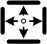
\includegraphics[width=0.08\textwidth]{feat1a.jpg}}
% \subfigure(WTRL){\label{fig:fig2a} 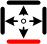
\includegraphics[width=0.08\textwidth]{feat2a.jpg}}
% \subfigure(WRLB){\label{fig:fig3a}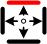
\includegraphics[width=0.08\textwidth]{feat3a.jpg}}
%
%   \subfigure(WTLB){\label{fig:fig4a}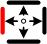
\includegraphics[width=0.08\textwidth]{feat4a.jpg}}
% \subfigure(WTRB){\label{fig:fig5a}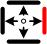
\includegraphics[width=0.08\textwidth]{feat5a.jpg}}
% \subfigure(WRB){\label{fig:fig6a}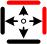
\includegraphics[width=0.08\textwidth]{feat6a.jpg}}
%
%     \subfigure(WTL){\label{fig:fig7a}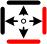
\includegraphics[width=0.08\textwidth]{feat7a.jpg}}
%   \subfigure(WLB){\label{fig:fig8a}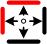
\includegraphics[width=0.08\textwidth]{feat8a.jpg}}
% \subfigure(WTR){ \label{fig:fig9a}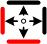
\includegraphics[width=0.08\textwidth]{feat9a.jpg}}
%  % \subfigure[Feature 'White\_3'.]{\label{fig:fig8}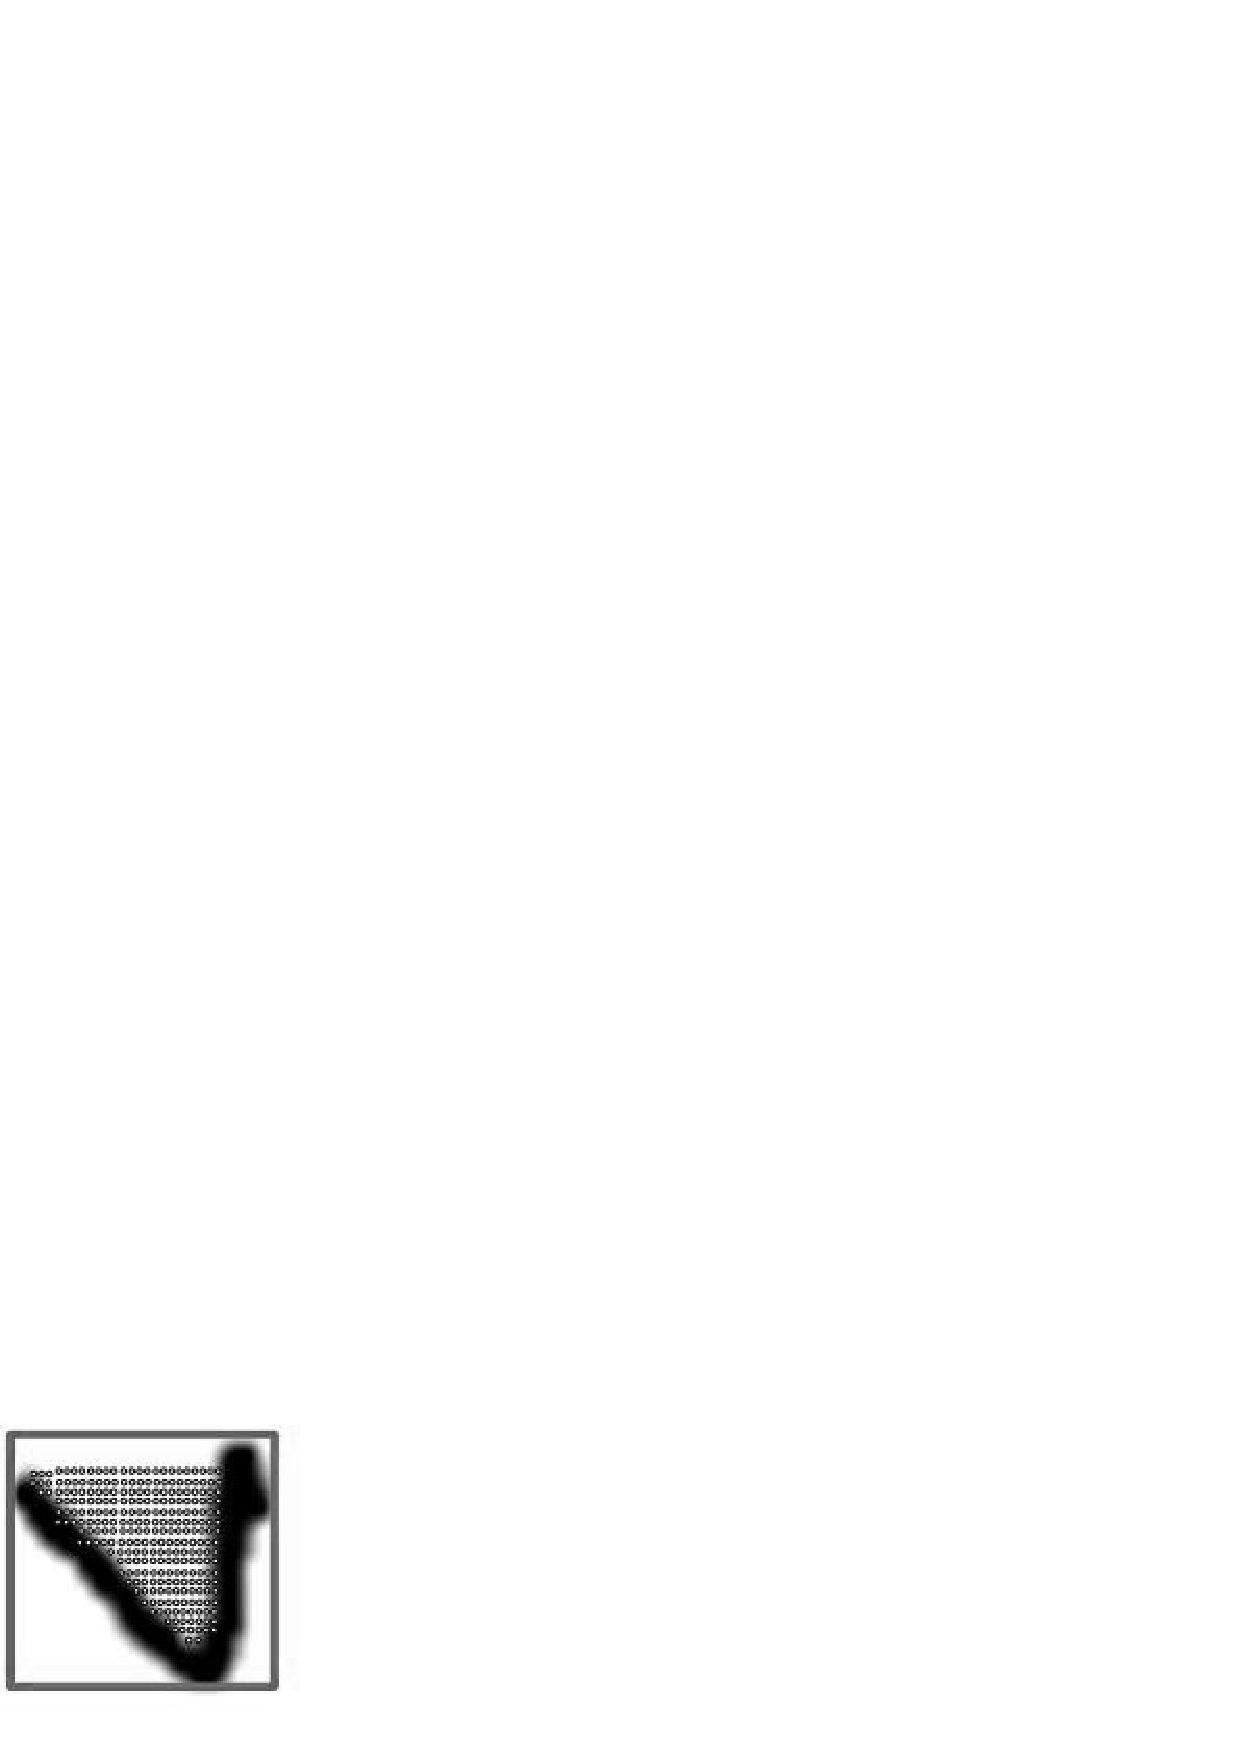
\includegraphics[width=0.13\textwidth]{figures/fig8.jpg}}
%  \caption{The concavity configrations used. Red for border pixel}
%  \label{fig:features}
% \end{figure}
\begin{figure}
\centering
 \subfigure[C1] {\label{fig:fig1a}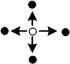
\includegraphics[width=0.08\textwidth]{feat1c.jpg}}
\subfigure[C2]  {\label{fig:fig2a} 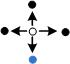
\includegraphics[width=0.08\textwidth]{feat2c.jpg}}
\subfigure[C3]  {\label{fig:fig3a}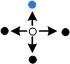
\includegraphics[width=0.08\textwidth]{feat3c.jpg}}

  \subfigure[C4]  {\label{fig:fig4a}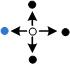
\includegraphics[width=0.08\textwidth]{feat4c.jpg}}
\subfigure[C5] {\label{fig:fig5a}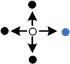
\includegraphics[width=0.08\textwidth]{feat5c.jpg}}
\subfigure[C6] {\label{fig:fig6a}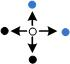
\includegraphics[width=0.08\textwidth]{feat9c.jpg}}

    \subfigure[C7] {\label{fig:fig7a}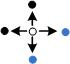
\includegraphics[width=0.08\textwidth]{feat8c.jpg}}
  \subfigure[C8] {\label{fig:fig8a}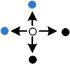
\includegraphics[width=0.08\textwidth]{feat7c.jpg}}
\subfigure[C9] { \label{fig:fig9a}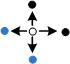
\includegraphics[width=0.08\textwidth]{feat6c.jpg}}
 % \subfigure[Feature 'White\_3'.]{\label{fig:fig8}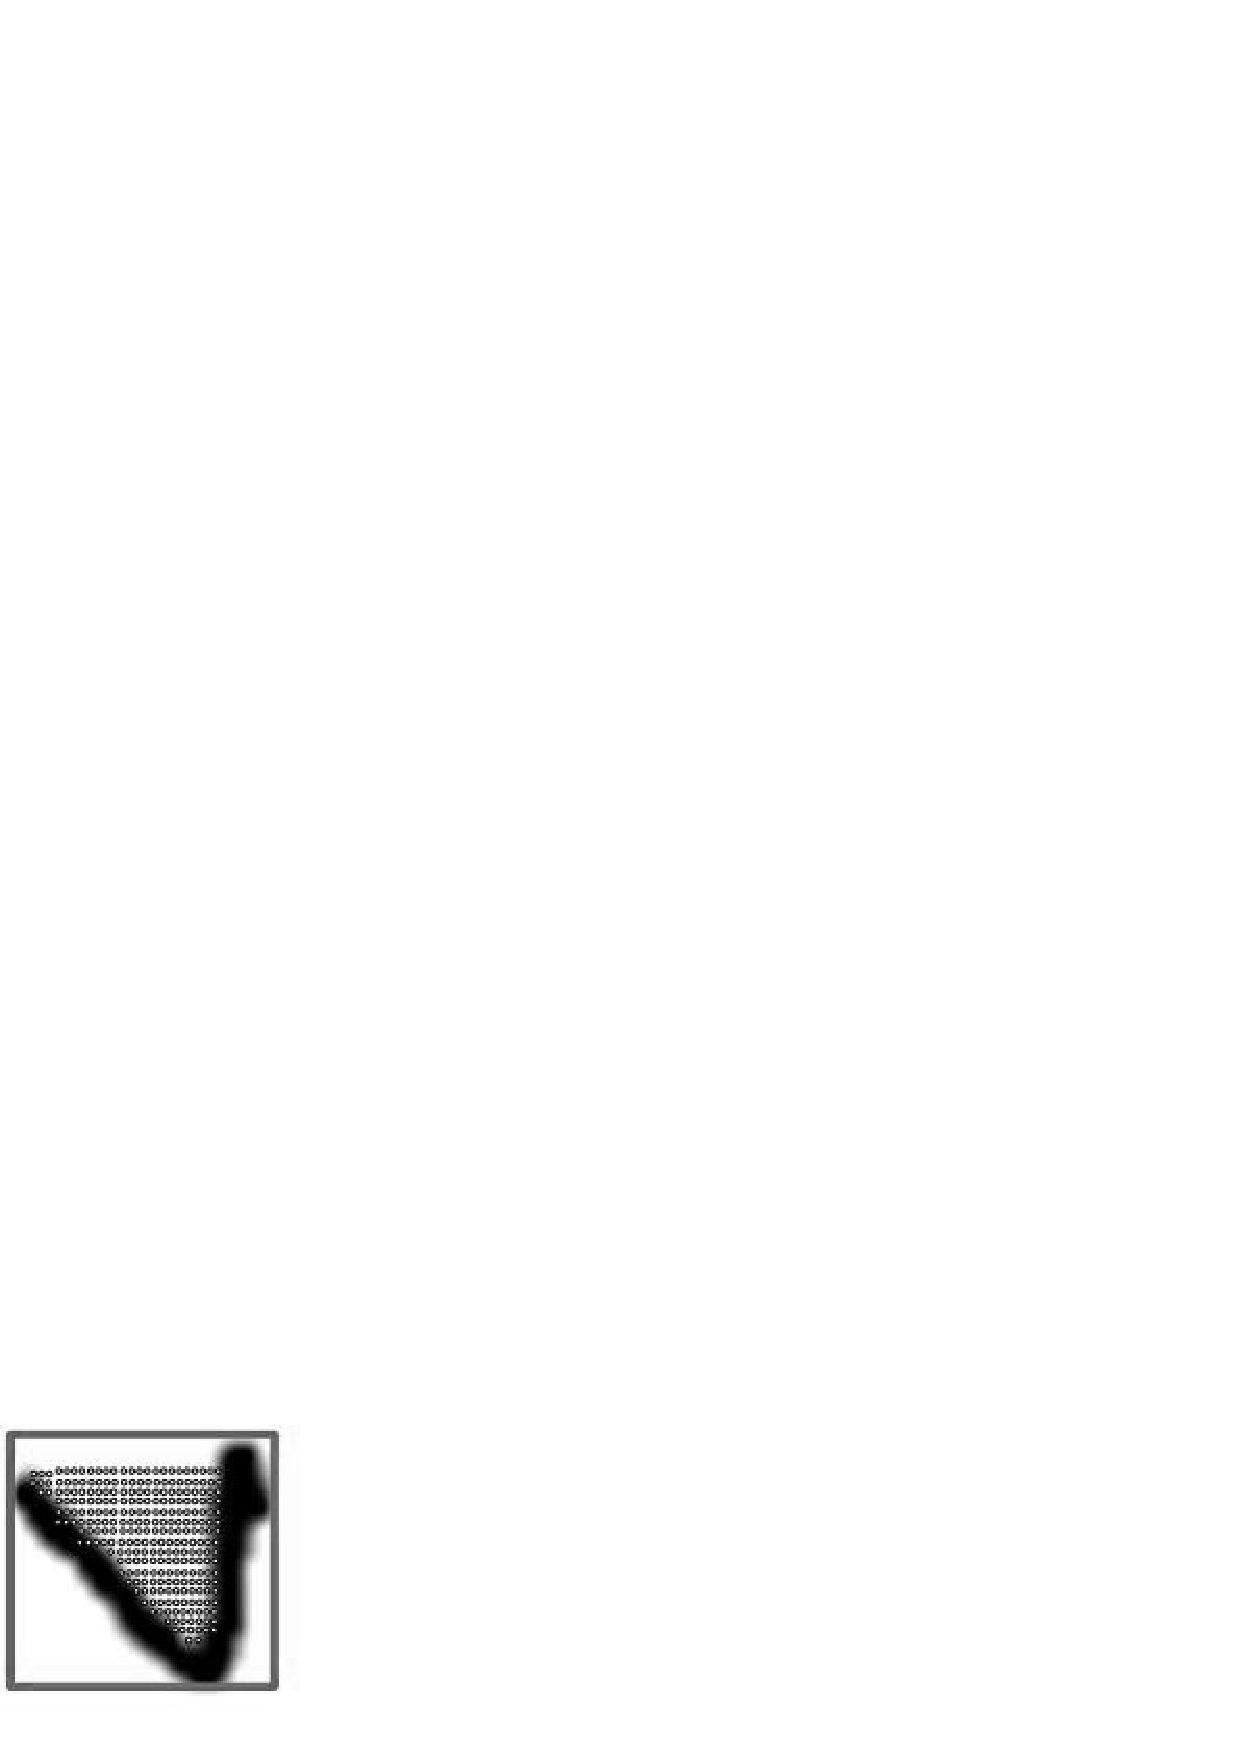
\includegraphics[width=0.13\textwidth]{figures/fig8.jpg}}
 \caption{The 9 concavity configurations. The blue pixel indicates the encounter of a bounding box}
 \label{fig:features}
\end{figure}

\subsection{Computing features from concavity maps}


The concavity configurations 1 to 9 are used to label each white pixel in the input digit. Figure  \ref{fig:VerticalDigit2} shows an example of an input digit 5 and the concavity map produced for the white pixels in the image. In the concavity map, each white pixel is labeled with its concavity configuration number from 1 to 9. The black pixels are labeled with 0 as they do not belong to any configuration

After producing the concavity map, features are extracted by dividing the image into strips in four directions (vertical, horizontal, right diagonal, and left diagonal) and the count of each of the nine concavity configurations in each strip is considered a feature as follows.
% Digit5image.jpg
%
% .jpg
\begin{figure}
	\centering
		%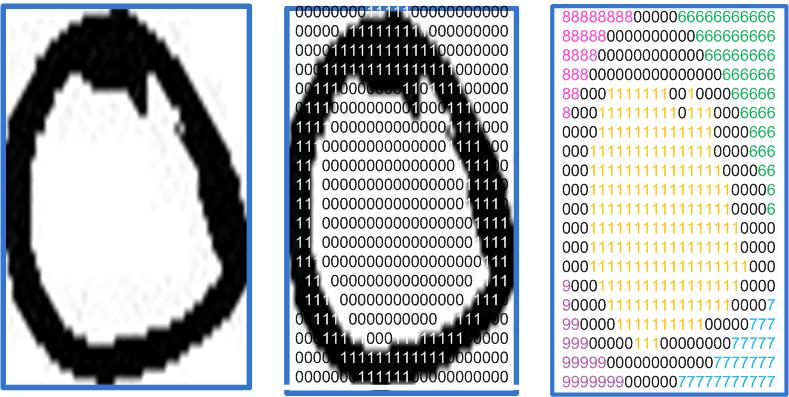
\includegraphics[scale=0.39]{Digit5Map.jpg}
		 \subfigure[Original Image] {\label{fig:5image}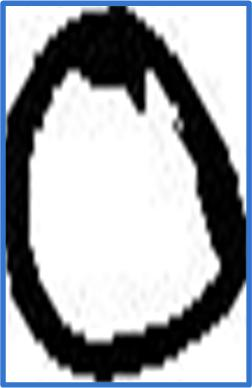
\includegraphics[width=0.2\textwidth]{Digit5image.jpg}}
\subfigure[Bitmap]  {\label{fig:5bitmap} 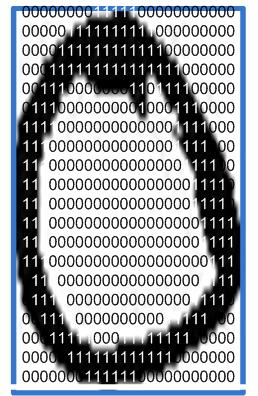
\includegraphics[width=0.2\textwidth]{Digit5Bitmap.jpg}}
\subfigure[Concavity Features]  {\label{fig:5concavity}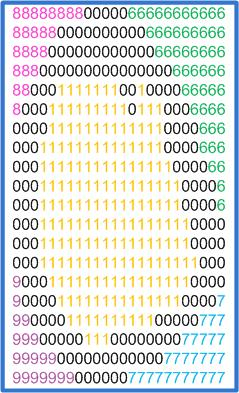
\includegraphics[width=0.2\textwidth]{Digit5MapOnly.jpg}}
	\caption[ Digit 5 ] {The Concavity Features of Digit 5 }
	\label{fig:VerticalDigit2}
\end{figure}


\begin{figure}
\centering
 \subfigure[Vertical] {\label{fig:figver}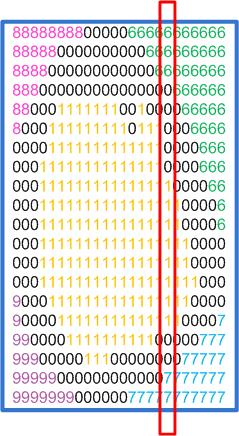
\includegraphics[width=0.15\textwidth]{Ver.jpg}}
\subfigure[Horizontal]  {\label{fig:fighorz} 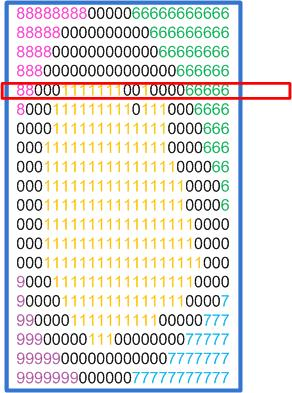
\includegraphics[width=0.17\textwidth]{horz.jpg}}
\subfigure[Left Diagonal]  {\label{fig:fig3left}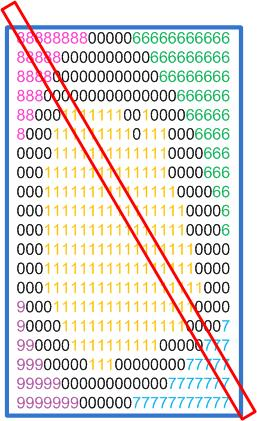
\includegraphics[width=0.17\textwidth]{left.jpg}}
 \subfigure[Right Diagonal]  {\label{fig:fig4right}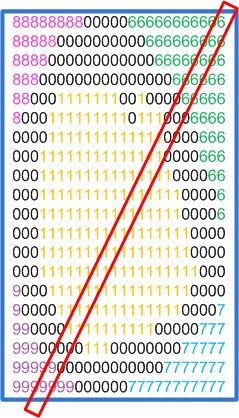
\includegraphics[width=0.15\textwidth]{right.jpg}}
 % \subfigure[Feature 'White\_3'.]{\label{fig:fig8}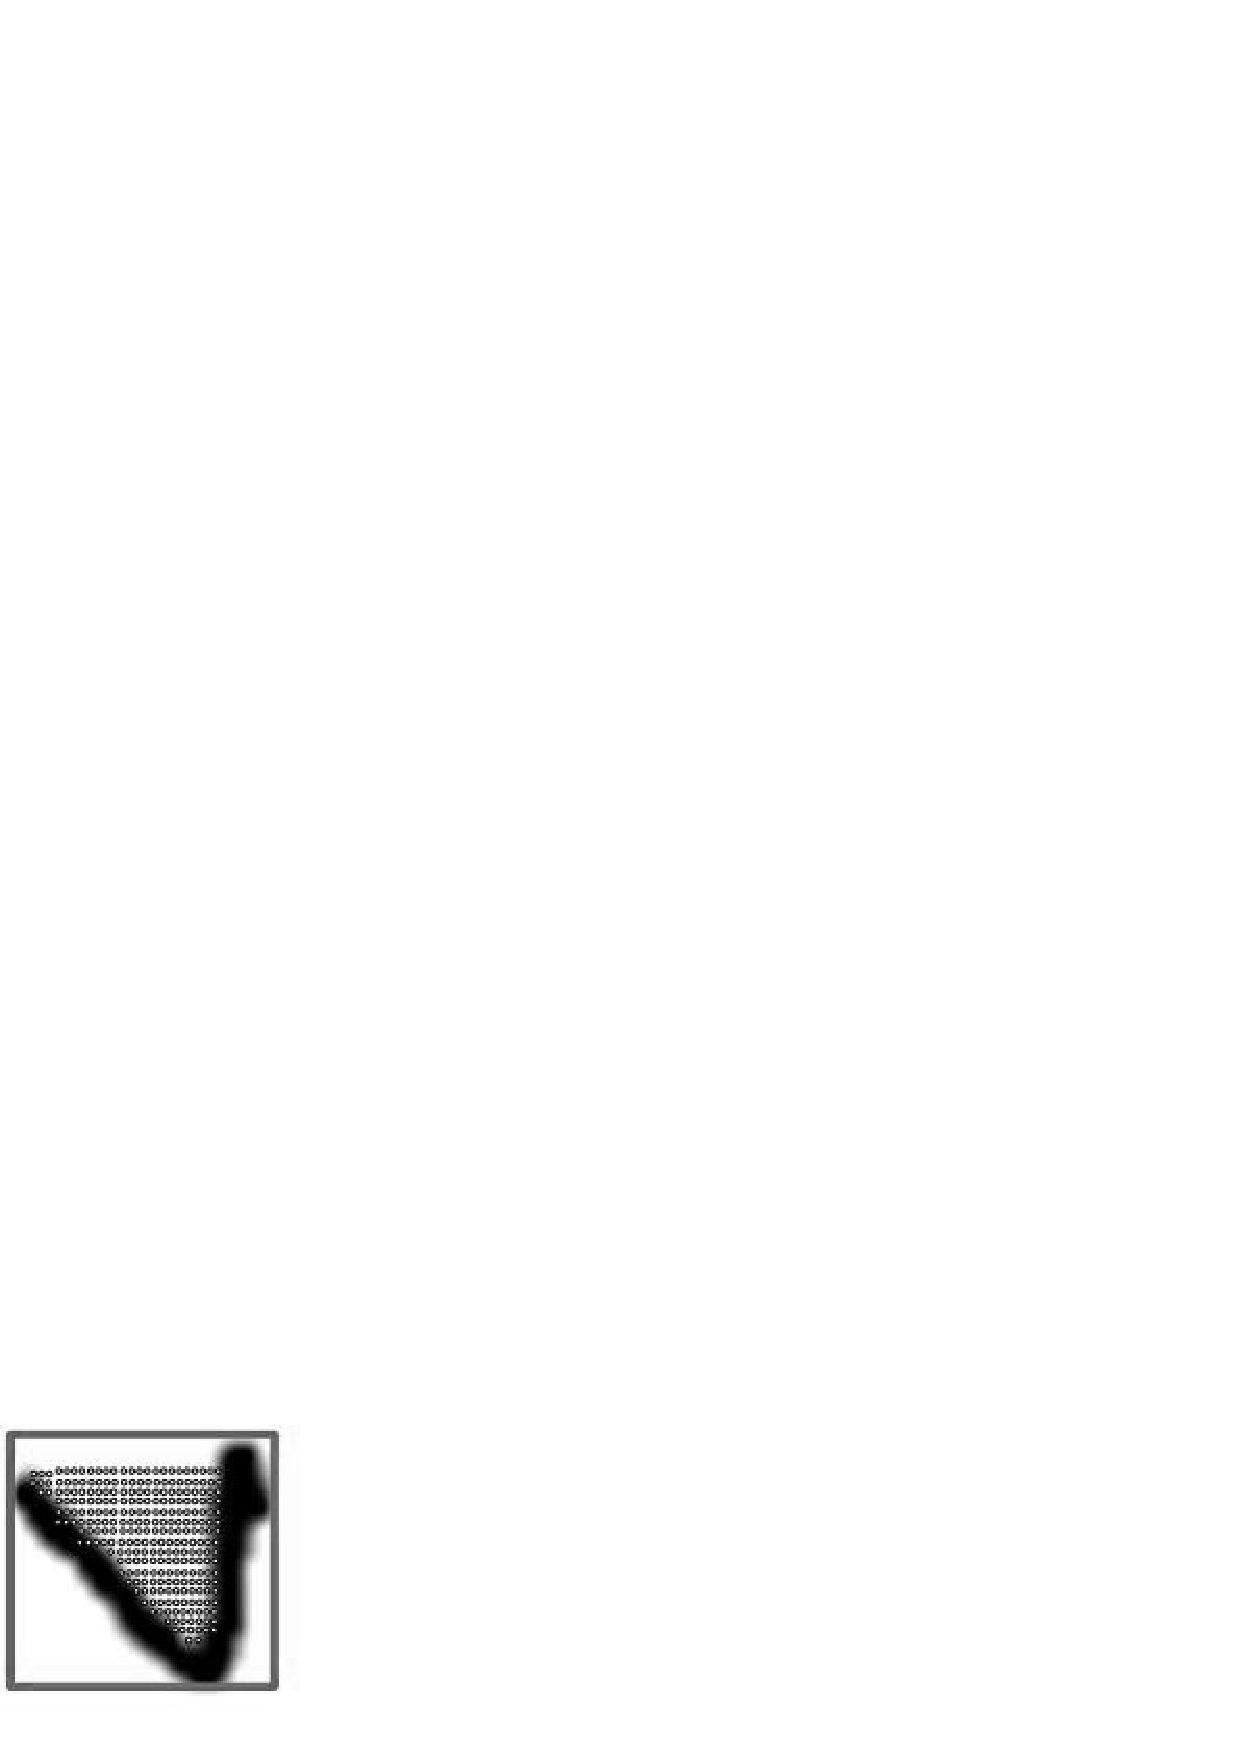
\includegraphics[width=0.13\textwidth]{figures/fig8.jpg}}
 \caption{ The Different Feature Orientation}
 \label{fig:featOrientation}
\end{figure}
\subsubsection{Vertical}
The concavity map is divided into vertical strips. The count of each concavity configuration in the strip is considered a feature. Figure \ref{fig:figver} shows an example of a vertical strip on a digit 5 concavity map. The feature vector for this strip is [ 8 0 0 0 0 3 2 0 0 ] because there are 8 pixels labeled with C1, 3 pixels labeled with C6, 2 pixels labeled with C7, and no pixels belonging to any other configuration.
%The concavity map is divided into vertical strips.  The count of each concavity configuration in the strip is considered a feature. Figure \ref{fig:figver} shows an example of a vertical strip on a digit 5 concavity map. The feature vector for this strip is [ 8 0 0 0 0 3 2 0 0 ] because there are 8 pixels labeled with C1, 3 pixels labeled with C6, 2 pixels labeled with C7, and no pixels belonging to any other configuration.
%The configuration map is traversed vertically to extract the count of each concavity configuration. Figure \ref{fig:figver} shows and example of a vertical strip on  digit 5  concavity map. The feature vector for this strip is [ 8 0 0 0 0  3  2  0 0  ] as it clearly shows that there is 8 pixels labeled with C1, 3 pixels labeled with C6, 2 pixels labeled with C7 and none in all other configurations. % labeled pixel
\subsubsection{Horizontal}

The concavity map is divided into horizontal strips. The count of each concavity configuration in the strip is considered a feature. Figure  \ref{fig:fighorz} shows an example of a horizontal strip on a digit 5 concavity map. The feature vector for this strip is [ 8 0 0 0 0 5 0 2 0 ] because there are 8 pixels labeled with C1, 5 pixels labeled with C6, 2 pixels labeled with C8, and no pixels belonging to any other configuration.
%The concavity map is divided into horizontal strips.  The count of each concavity configuration in the strip is considered a feature. Figure \ref{fig:fighorz} shows an example of a horizontal strip on a digit 5 concavity map. The feature vector for this strip is [  8 0 0 0 0 5 0 2 0 ] because there are 8 pixels labeled with C1, 5 pixels labeled with C6, 2 pixels labeled with C8, and no pixels belonging to any other configuration.
%The configuration map is traversed horizontally to extract the count of each concavity configuration. Figure \ref{fig:fighorz} shows and example of a horizontal strip on  digit 5  concavity map. The feature vector for this strip is [ 8 0 0 0 0 5 0 2 0 ] as it clearly shows that there is 8 pixels labeled with C1, 5 pixels labeled with C6, 2 pixels labeled with C8 and none in all other configurations. % labeled pixel
\subsubsection{Left Diagonal}
%The concavity map is divided into left diagonal strips.  The count of each concavity configuration in the strip is considered a feature. Figure \ref{fig:fig3left} shows an example of a left diagonal strip on a digit 5 concavity map. The feature vector for this strip is [11 0 0 0 0  0  3  3  0 ] because there are 11 pixels labeled with C1, 3 pixels labeled with C7, 3 pixels labeled with C8, and no pixels belonging to any other configuration.

The concavity map is divided into left diagonal strips. The count of each concavity configuration in the strip is considered a feature. Figure \ref{fig:fig3left} shows an example of a left diagonal strip on a digit 5 concavity map. The feature vector for this strip is [11 0 0 0 0 0 3 3 0 ] because there are 11 pixels labeled with C1, 3 pixels labeled with C7, 3 pixels labeled with C8, and no pixels belonging to any other configuration.
%The configuration map is traversed using left diagonal to extract the count of each concavity
\subsubsection{Right Diagonal}
%The concavity map is divided into right diagonal strips.  The count of each concavity configuration in the strip is considered a feature. Figure \ref{fig:fig4right} shows an example of a right diagonal strip on a digit 5 concavity map. The feature vector for this strip is [ 10  0  0  0  0 5 0 0 2 ] because there are 10 pixels labeled with C1, 5 pixels labeled with C6, 2 pixels labeled with C9, and no pixels belonging to any other configuration.
 The concavity map is divided into right diagonal strips. The count of each concavity configuration in the strip is considered a feature. Figure  \ref{fig:fig4right} shows an example of a right diagonal strip on a digit 5 concavity map. The feature vector for this strip is [ 10 0 0 0 0 5 0 0 2 ] because there are 10 pixels labeled with C1, 5 pixels labeled with C6, 2 pixels labeled with C9, and no pixels belonging to any other configuration.



It has to be noted that the width of the strips used to extract the features in the different directions could be of any number of pixels. The strips used in the example shown in Figure \ref{fig:featOrientation} have widths of one pixel. A validation set has been used to find the best empirical width for the strips as explained in Section \ref{sec:Results}. Another note is that the feature vector obtained for each strip is normalized by dividing the number of pixels of every concavity configuration by the total number of white pixels in the strip


\subsection{Digit Zero Problem}
\label{sec:ZeroProblem}
The Arabic Digit zero '0' is very difficult to recognize because there is no specific way to write it, as it is only like a decimal point. Figure \ref{fig:zerosize} shows different samples of the Arabic Digit '0'. The figure clearly shows that the digit has no specific way of writing and it usually confuses with other digits especially Arabic digits '1' and '5'. The most discriminating feature for the digit '0' over the other digits is its small size. Figure \ref{fig:zeroVersusOther} shows the average size of Digit '0' versus other Arabic digits. Thus, to solve the digit zero problem we have added a feature $area$  that describes the size of the bounding box of the digit. Another feature  $height/width$  has been added to distinguish digit '0' from digit '1'. Those two features have significantly increased the recognition rate of the zero.

%The Arabic Digit zero '0' is very difficult to recognize because there is no specific way to write it, as it is only like a decimal point. Figure\ref{fig:zerosize} shows different samples of the Arabic Digit '0'. The figure clearly shows that the digit has no specific way of writing and it usually confuses with other digits especially Arabic digits '1' and '5'. The most discriminating feature for the digit '0' over the other digits is its small size. Figure  \ref{fig:zeroVersusOther} shows the average size of Digit '0' versus other Arabic digits. Thus, to solve the digit zero problem we have added a feature $area$ that describes the size of the bounding box of the digit. Another feature $height/width$ has been added to distinguish digit '0' from digit '1'. Those two features have significantly increased the recognition rate of the zero.

%The Arabic Digit zero '0' is very difficult to recognize because it has no specific way to write it, as it is only like a decimal point. Figure \ref{fig:zerosize} shows different samples of the Arabic Digit '0'. The figure clearly shows that the digit has no specific way of writing  and it usually confuses with other digits especially Arabic digits '1' and '5'. The most discriminating feature for the digit '0' over the other digits is its size and number of points used to write it. Figure \ref{fig:zeroVersusOther} shows the average size of Digit '0' versus other Arabic digits. Since digit '0' is written in a small area and random direction, it is better be recognized separately


%The main feature that discriminate the zero digit the the remaining of the Arabic digits is size information.  Thus, to solve the digit zero problem we add two features that describe size of the digit. The features are  $height/width$ and  $area$ of the bounding box before the resizing step. These two feature increase the recognition rate of the zero significantly. % and two more features are added to the feature vector of each classifier.

 \begin{figure}
	\centering
		\includegraphics[scale=0.35]{Zero0}
	\caption[Arabic '0' Digits ] {Different samples of the Arabic Digit '0'}
	\label{fig:zerosize}
\end{figure}


 \begin{figure}
	\centering
		\includegraphics[scale=0.2]{Zero1}
	\caption[Arabic '0' Digits Versus Other digits] {The difference in size between digits '0' and other digits..}
	\label{fig:zeroVersusOther}
\end{figure}


%Adding the final two features makes the feature vector for the classifier composed of 47 features: 45 concavity features and 2 size features

%Adding the final two features makes the feature vector for the classifier 47 features which include 45 concavity features and 2 size features.


\section {Classification}
\label{sec:classification}
In the proposed system a classifier is used for the concavity features obtained from each of the four orientations: horizontal, vertical, left diagonal, and right diagonal. Figure  \ref{fig:block} shows the block diagram of the system. First, the feature vector for every orientation is computed then introduced to the corresponding classifier. To get a single decision from the system we employ decision fusion methods to reach the final classification. The next sections describe the classifiers used and the fusion methods.

%The final stage of the system is the classification stage where the computed feature vectors are introduced to the classifier for recognition. Figure \ref{fig:block} shows the block diagram of the system. First, the feature vector is computed then introduced to four different classifiers, one classifier for each orientation. To get a single decision from the system we employ a decision fusion method to reach the final classification. The next sections describe the  classifiers used and the fusion methods.

%The final step of the system is the classification stage where the computed feature vectors are introduced to the classifier to label each image with the correct digit. Figure \ref{fig:block} shows the block diagram of the system. Firstly, the feature vector is computed then introduced to four different classifier, one classifier for each orientation. To get a single decision from the system we employ a decision fusion method to reach the final classification. The next sections describe in details the single classifier used and the fusion methods. %the

 %The system then uses a decsion fusion mechanizem to reach a final decision on the digit label. Figure \ref{fig:block} shows the block diagram of the system.
 \begin{figure}
\centering
\label{fig:block}
\includegraphics[width=0.45\textwidth]{BlockDiagram.jpg}
 \caption{The Block diagram }
\end{figure}


\subsection{Single Classifiers}

%The input of the feature extraction method is four different feature vector based on orientation used. A classifier is used for each orientation which means that the feature vector for each classifier consist of  $9\timesn$ concavity map. To simplify the classification we use simple one versus one (OVO) Support Vector Machine (SVM) using linear kernel classifier. Since the SVM is a binary classifier we used One versus one configuration for the classifiers which requires
The output of the feature extraction stage is four different feature vectors for the four different orientations used. A classifier is used for each orientation. To simplify the classification we use simple one versus one (OVO) Support Vector Machine (SVM) with linear kernel classifier. Since the SVM is a binary classifier, the one versus one classification requires $\frac{n(n-1)}{2}$ classifiers for $n$ classes. The final decision of the classification in a one versus one classifier can be obtained using simple majority voting. Unfortunately, this method does not generate the confidence measure for each class needed in the classifier fusion step. Various methods can be used to generate such probability or confidence measure from pairwise classifiers. One of the popular methods is introduced in \cite{pairwise22} where $p_i$ probability of sample $x$ to belong to class $i$  is computed using the following equation :

%The output of the feature extraction stage is four different feature vectors for the four different orientations used. A classifier is used for each orientation. To simplify the classification we use simple one versus one (OVO) Support Vector Machine (SVM) with linear kernel classifier. Since the SVM is a binary classifier, the one versus one classification requires $\frac{n(n-1)}{2}$ classifiers for $n$ classes. The final decision of the classification in a one versus one classifier can be obtained using simple  majority voting. Unfortunately, this method does not generate a confidence measure for each class which is needed in the classifier fusion step. Various methods can be used to generate such probability or confidence measure from pairwise classifiers. One of the popular methods is introduced in \cite{pairwise22} where $p_i$ probability of sample $x$ to belong to class $i$  is computed using the following equation :
%
% The final decision of the classification can be extraction using various method. One of the simple methods is majority voting.  Unfortunately, this method does not generate a confidence measure for each class which we need in the classifier fusion step. Various methods were used to generate such  probability or  confidence measure from pairwise classifiers. One of the popular methods used is introduced in \cite{pairwise22} where
%  \[
% p_i=\frac{1}{r_{ij}k-1}
% \]
\[
P_i(x)  = \frac{1}{{\sum\limits_{j = 1,j \ne i}^K {\frac{1}{{r_{ij}(x) }} - (K - 2)} }}
\]

where $r_{ij}(x)$   is the probability of the tested pattern $x$ to be of class $i$, where the used classifier is the one responsible for separating class $i$ from class $j$  and $k$ is the number of classes.
%  To  for each feature orientation. These meanThe horizontal feature are computed using Single SVM and hence vice,. Hence, there are four classifiers on for each orientaition. Each classifier has 9xs where s is the number of strips in each orientation.
%
% Each orientation is presented to a single classifier. The SVM classsifier is used beacuse it represents a superior recognitoin rate over all classifiers. The linear kernel was used to simply the training and testing procedures.  Since the SVM is a binary classifier we used One versus one configuration for the classifiers which requires $\frac{n(n-1)}{2}$ classifiers for $n$ classes.



\subsection{Fusion Methods}
Fusion methods can be divided into three main categories: label based, rank based, and soft margin or fuzzy based methods. The label based method are usually based on the final label of base classifiers like the majority voting fusion. The rank based method uses the decision values of base classifiers to rank using various fixed rules to get the final decision for the system. The soft margin and fuzzy based methods use the output decision values of the base classifiers as a pattern recognition problem and try to detect the correct pattern. Methods like Bayes and neural network fusion are considered the most widely used fusion methods based on this type  \cite{Farah2005,Ruta2000,Denoeux2000}.

%Fusion methods can be divided into three main categories Label based, Rank based and soft margin or fuzzy based methods. The label based method are usually based on the final label of base classifiers like the majority voting fusion. The rank based method uses the decision values of base classifier to rank uses various fixed rule to get the final decision value for the system. The soft margin and fuzzy based methods tries to use the output decision values  of the base classifier as a pattern recognition problem and tries to try to detect the correct pattern. Methods like Bayes and neural network fusion is considered the most fusion method based on this type. .



%The four base classifiers generate a set of normalized probability for each class $P_i(x)$ for a given input sample $x$. These probabilities are as input the fusion methods.

The four base classifier generate the posterior probabilities $P_{ij}(x), i = 1,c; j = 1,k$ for $c$ classifiers and $k$ classes is computed for test sample $x$. A fusion method will  combine them to a new set of probability  $q_j(x)$ which can be used for the final classification. Let $q_j(x)$ be computed by :
\[
q_j(x)=rule_i\left(P_{ij}(x)\right)
\]

The final classification is made by:
\[
\phi(x)=\max\limits_j(q_j(x))
\]
The rules used to compute $q_j(x)$ are summarized below:
%A single classifier selects the class which maximizes the normalized probability. The classifiers, used to find each  for a given test sample x, are summarized below:

%In the next section we describe the various fusion method tested in the system.
% There is various rules for the fuision, let the  is the $ p_{ij}(x)$ probabity (decision) value of sample $x$ with respect to class $i$ where $i=1\dots,c$ and $c$ is number of classes and in this case $c=10$.
%  \[
%  p_{ij}(x)=prob(\omega_i|C_{ij}(x))
%  \]
% where $C_{ij}(x)$ is some numerical outcome of classifier $j$ for class $i$. The most known simple fixed rules to combine basoc classifiers $C_i(x), i=1, ..., c$ into a combining classification problem of  $classifierQ_i(x)=$ will be presented by.
%
%
% Once the posterior probabilities {pij(x), i = 1,m; j = 1,c} for m classifiers and c classes is computed for test object x, they have to be combined into a new set qj(x) which can be used for the final classification. qj(x) is computed by:
% q j'(x) = rulei(pij(x)) q j'(x)
% q j(x) =
%   pj(x) = 1 j
% The final classification is made by:  (x) = argmaxj(q j(x))
% Three combining rules are used for rule in (2)
\subsubsection{Product rule}
% This rule is good if the individual classifiers are indepen-
% dent, i.e. that the outcomes of Cij(x) for random x are inde- pendent for fixed i (class) and variable j (classifier). This is hardly ever the case. An example may be found by two clas- sifiers computed for different feature spaces that are entirely unrelated, e.g. based on face images and voices assuming that within a class the feature distributions in the two spaces are independent.
The base classifier generate a normalized probability value for each class, then all the normalized value are multiplied per class. The final class is determined by the class with high probability product. The rule can be defined as :
\[
q_j(x)=\prod\limits_i{p_{ij}(x)}
\]

\subsubsection{Majority Vote rule}
This fusion method is one of the most widely  used label based fusion.  It simply counts the votes for each class over the input classifiers selecting the class with the majority of votes. It can be represented as %This fusion method is one of the most used label based fusion, as it simply by counting the votes for each class over the input classifiers.Selectin the class with the majority of votes. It can be represented as
\[
q_j(x)=l(\max\limits_i(p_{ij}(x))=i))
\]
where $I(y)=1$ if $y$ is true and $o$ otherwise.
\subsubsection{Sum rule}
 The base classifier generates a normalized probability value for each class, then all the normalized value are summed per class. The final class is determined by the class with the highest probability sum. The rule can be defined as
 %The base classifier generate a normalized probability value for each class, then all the normalized value are summed per class. The final class is determined by the class with high probability product. The rule can be defined as :
\[
q_j(x)=\sum\limits_i{p_{ij}(x)}
\]
\subsubsection{Maximum rule}
The maximum rule chooses the class that has the highest normalized probability among the base classifiers.%The maximum rule chose the class that has the highest normalized probability from the base classifiers.
\[
q_j(x)=\max\limits_i{p_{ij}(x)}
\]
\subsubsection{Minimum rule}
Similar to Max rule but chose the classifier with min value per class. This means that it choose the classifier with the lest objection against a certain class.%Similar to Max rule but chose the classifier with min value per class. This means that it choose the classifier with the lest objection against a certain class.
\[
q_j(x)=\min\limits_i{p_{ij}(x)}
\]
\subsubsection{Median and Mean rules}
  Similar to sum rule but the decision is based on the median or the mean of the classifiers output rather than the sum of the probabilities.%Similar to sum rule but the decision is based on the median or the mean of the classifiers output rather than the sum of the probabilities.



\subsubsection{Weighted Sum rule}
 The base classifiers generate normalized probability values for each class, then all the normalized values are summed per class. The final class is determined by the class with the highest probability product. The rule can be defined as :
 %The base classifier generate a normalized probability value for each class, then all the normalized value are summed per class. The final class is determined by the class with high probability product. The rule can be defined as :
\[
q_j(x)=\sum\limits_i{p_{ij}(x)*w(i)}
\]
where $w(i)$ is the weight of the classifier $i$.



\subsubsection{Borda Count}
 One of the most used ranking based fusion methods is the Borda Count (BC). It is defined as mapping from the base classifier ranking to a single final ranking. The final ranking of each class  $i$  is defined as the sum of number of classes that are ranked below class $i$  in each classifier $j$ . The Borda count is considered a generalization of the majority vote rule.
%One of the most used ranking based fusion is the Borda Count (BC). It define as mapping from the base classifier ranking to a single final ranking. The final ranking of each class $i$ is defined as the sum of number of classes that are ranked below class $i$ in each classifier $j$.  The Borda count is considered a generalization of the majority vote rule.
% Borda Count (BC) is an example of group consensus functions, defined as a mapping from a set of individual rankings to a combined ranking leading to the most relevant decision [1], [2]. For a particular class k
% c Borda Count B )(ck number of classes ranked below class k
% is defined as a sum of the c by each
%
% classifier. The magnitude of the BC reflects the level of agreement that the input pattern belongs to the considered class. To a certain degree the BC can be treated as a generalization of the majority-voting rule and for a case of two classes problem it is exactly reduced to the majority vote.

\subsubsection{Neural Network fusion}
 %A neural network can be trained to perform a mapping of input decision from $c$  base classifiers to the output of  $k$ classes that can be used to reach a final decision. The training of the neural network is done through an iterative learning process.
 A neural network can be trained to perform a mapping of input decision from $c$  base classifiers to the output of  $k$ classes that can be used to reach a final decision. The training of the neural network is done through an iterative learning process
% A neural network can be trained to perform as a mapping of input decision from $c$ base classifiers to the output of $k$ classes that can be used to reach a final decision. The training of the neural network is done through an iterative learning process. In our system we used a Multilayer perceptron (MLP) neural network to learn the output decision of our four classifiers. The output of the neural network is considered the final label of the system. The MLP consist of one hidden layer and 80 hidden neurons learned using back backpropagation algorithm.


\section {Experiments and Results}
\label{sec:Results}
The experiment are performed on the ADBase database which consist of 70,000 handwritten digits collected form 700 different writers. The dataset is divided into 60,000 samples for the training set and 10,000 samples for the test set. The classifiers' parameters are optimized using a validation set of 10,000 samples taken from the training set. The validation set has been used to obtain the best number of strips $n$ (5, empitrically) in each of the four orientations, the classifiers' parameters, and for training the neural network for fusion of the classifiers.
%The experiment are performed on the ADBase database which consist of 70,000 handwritten digits collected form 700 different writers. The dataset is divided into 60,000 samples for the training set and 10,000 samples for the test set. The classifiers' parameters are optimized using a validation set of 10,000 samples taken from the training set. The validation set has been used to obtain the best number of strips $n$(5, empitrically), classifier parameters, and training the neural network for fusion of the classifiers.


The number of features in  the feature vector obtained for every orientation is the number of features  per strip times the number of strips. This amounts to 45 (9 concvavity features * 5 strips) features. This is in addition to the two size features used to disstinguish digit '0' from all other digits. Thus, the number of features used for each of the four classifiers is 47 (45+2).

\subsection{Experiments on Separate Classifiers}

 Table \ref{tab:numberOfstrips} shows the results of all the single classifiers on each feature orientation. The results show that the horizontal orientation reports the highest accuracy. This observation may be due to Arabic Digits having more visually discriminative features on the horizontal orientation than on any other orientation.

 \begin{table}
 \centering
% \begin{center}
\caption[Single Classifier Results]{Single Classifier Results}
%\scalebox{0.8}{{
 \begin{tabular}{|c|c|}
  \hline
Classifier & Recognition rate \\  \hline \hline
Horizontal &99.24	 \\ \hline
Vertical &99.07 \\  \hline
Right diagonal &98.79\\  \hline
Left Diagonal  & 98.85\\  \hline

\end{tabular}
\label{tab:numberOfstrips}
\end{table}
%As mentioned in section \ref{sec:classification}


\subsection{Experiment for Fusion Methods}

Table \ref{tab:fusion} shows the results of the different fusion methods used to combine the results of all the four basic classifiers. The table shows the final system results after the fusion rules are applied. The results show that the Mean, Median, Majority vote, Borda Count, and neural network fusion methods give comparable results. The neural network result is the best but it needs a repetitive training which increases the complexity of the system. The neural network used is a multilayer perceptron (MLP) neural network to learn the output decision of our four classifiers. The output of the neural network is considered the final label of the system. The MLP consists of one hidden layer and 80 hidden neurons using the back propagation algorithm.



 \begin{table}
 \centering
% \begin{center}
\caption[Result of different fusion methods]{ Result of different fusion methods}
%\scalebox{0.8}{{
 \begin{tabular}{|c|c|c|c|}
  \hline
Fusion Method	& Recognition Rate		 \\  \hline
Majority Voting	&99.32	\\  \hline
	Sum	&99.32	\\ \hline
	Product	&99.29		\\   \hline
	Weighted sum	&99.31		\\  \hline
	 Borda Count	&99.32	\\ \hline
	Mean	&99.32	\\ \hline
	Median	&99.33		\\ \hline
	Max	&99.18		\\ \hline
	Min	&99.21		\\ \hline
	Neural Network 	& 99.36 \\ \hline
\end{tabular}
\label{tab:fusion}
\end{table}






Table \ref{tab:confusion} shows the system final confusion matrix with the neural network used at the fusion stage.

 \begin{table}[h]
 \centering
% \begin{center}
\caption[First Stage result table]{ Confusion Matrix }
%\scalebox{0.8}{{
 \begin{tabular}{|p{0.3in}|c|c|c|c|c|c|c|c|c|c|c|}
  \hline
 Actual Predict & 0 &1&2&3&4&5&6&7&8&9 \\   \hline
0 & 0 & 2 & 0 & 0 & 0 & 2 & 1 & 0 & 0 & 0 \\ \hline
1& 2 & 0 & 1 & 0 & 0 & 0 & 1 & 0 & 0 & 0 \\ \hline
2& 0 & 1 & 0 & 2 & 4 & 2 & 0 & 0 & 1 & 1 \\ \hline
3& 0 & 0 & 0 & 0 & 0 & 0 & 0 & 2 & 0 & 0 \\ \hline
4& 1 & 1 & 4 & 2 & 0 & 1 & 0 & 0 & 0 & 1 \\ \hline
5& 11 & 0 & 1 & 0 & 0 & 0 & 0 & 1 & 0 & 0 \\ \hline
6 & 0 & 0 & 1 & 1 & 0 & 0 & 0 & 1 & 2 & 3 \\ \hline
7 & 0 & 0 & 0 & 0 & 1 & 1 & 0 & 0 & 0 & 0 \\ \hline
 8& 1 & 2 & 0 & 0 & 0 & 1 & 0 & 0 & 0 & 0 \\ \hline
 9& 0 & 0 & 0 & 0 & 1 & 1 & 1 & 1 & 1 & 0 \\ \hline
% 0&0	&0&	0&	0 &	3&	1&	0&	0&	0 \\   \hline
% 1&2&	0 &	2 &	3&	1&	0&	0&	0&	1	 \\   \hline
% 2&0&	9 &	0 &	0&	0&	0&	0&	0&	3	 \\   \hline
% 3&0&	0 &	0 &	0&	0&	0&	0&	0&	1	 \\   \hline
% 4&0&	0 &	10 &	1&	0&	0&	0&	0&	2	 \\   \hline
% 5&0&	0 &	0 &	0&	0&	0&	0&	1&	2	 \\   \hline
% 6&14&	0 &	1 &	0&	0&	1&	0&	0&	0	 \\   \hline
% 7&0&	0 &	0 &	0&	0&	1&	0&	0&	0	\\   \hline
% 8&0&	4 &	0 &	1&	1&	3&	0&	0&	0	\\   \hline
% 9&1&	0 &	0 &	0&	1&	0&	0&	0&	0	\\   \hline
\end{tabular}
\label{tab:confusion}
\end{table}




\subsection{Comparison to Other Systems}
We have compared the results obtained by the proposed system with previous results on the same Arabic handwritten digits database using linear SVM as reported in \cite{IjdarSherifPaper,Abdelazeem2009}. The results are given in Table \ref{tab:AccuraciesOfClassifierFeaturesPairsOnMADBase} for the proposed system and for several other feature extraction techniques. Comparing the results clearly reveals the superiority of the proposed system with a recognition rate of 99.36\% over all previously reported methods. Moreover,  concavity features in the horizontal orientation alone without any classifier fusion produces 99.24\% recognition rate (see Table \ref{tab:fusion}) which is superior to most previous feature extraction methods.

%The results are shown in Table \ref{tab:AccuraciesOfClassifierFeaturesPairsOnMADBase}. Using concavity features alone without any fusion produces competitive results (99.24\%) with previous feature extraction methods as shown in Table \ref{tab:confusion}. Using classifier fusion along with concavity features makes the proposed system (99.36\%) superior to all previously reported systems.









% \begin{table*}
% 	\centering
% 		\caption{Accuracies of classifier/features pairs on MADBase}
% 	\label{tab:AccuraciesOfClassifierFeaturesPairsOnMADBase}
% 	%\scalebox{0.99}{
% 		\begin{tabular}{|l|c|c|c|c|c|c|c|c|c|c|}
% 		 \hline
%   Feature	& KNN	& Parzen	& NN	&PCA + Quad	&Linear SVM	& SVM RBF 	&GC	&Fisher \\ \hline
% Gradient&	98.9	&98.92	&98.98	&99.11	&99.03&	99.18&	97.94	&98.27	\\ \hline
%
% 	Kirsch &	98.14	&98.02	&98.5	&98.27&	98.82&	98.87&	97.25	&97.57\\ \hline
% 		Local Chain	&95.41&	94.32	&96.12	&96.46&	96	&97.08&	93.29&	95.72\\ \hline
% Wavelet	&98.56	&98.34	&98.46	&98.03	&97.2&	98.85&	96.23	&95.53\\ \hline
%
% 		\end{tabular}
% 		%}
% \end{table*}
\begin{table}
	\centering
		\caption{Accuracies of different features using  Linear SVM}
	\label{tab:AccuraciesOfClassifierFeaturesPairsOnMADBase}
	%\scalebox{0.99}{
		\begin{tabular}{|l|c|c|c|c|c|c|c|c|c|c|}
		 \hline
  Feature	& Recognition Rate \\ \hline
  Gradient & 99.18\\ \hline
Gradient+size&	 99.22	\\ \hline

	Kirsch &	99.06 \\ \hline
		Local Chain	& 98.32\\ \hline
Wavelet	&97.73 \\ \hline
Domain specific & 99.25\\ \hline
Proposed System & 99.36 \\ \hline

		\end{tabular}
		%}
\end{table}

\section{Conclusion}
\label{sec:Conclusion}
  In this paper we introduced a system that recognizes Arabic handwritten Digits with 99.36\% efficiency. The system uses 9 different concavity features. The features are extracted in four orientations: horizontal, verital, righ diagonal, and left diagonal. Four different classifiers are then used, one for each orientation. The classifier outputs are then passed through a classifier fusion system. Different types of fusion have been used to achieve a final recognition accuracy of 99.36\%.


Further work can be done in order to investigate the efficiency of the proposed concavity features in the problem of Arabic characters recognition. Moreover, the proposed features can be used with different classifiers like hidden Markov model (HMM) as the strips can be converted into HMM observations.


%In this paper we introduced a system that recognizes Arabic handwritten Digits with 99.36\% efficiency. The system uses 9 different concavity features. The features are extracted in four directions: horizontal, verital, righ diagonal, and left diagonal. Four different classifiers are then used, one for each direction. The classifier outputs are then passed through classifier fusion system. Different types of fusion have been used to achieve final recognition accuracy of 99.36\%.

%Further work can be done in order to investigate the efficiency of the proposed concavity features in the problem of  Arabic characters recognition. Moreover, the proposed features can be used with different classifiers like hidden Markov model (HMM) as the strips can be converted to HMM observations.




%develop new features based on structural information.
\bibliographystyle{IEEEtran}
\bibliography{IEEEabrv,mybibfile,LibraryFinal,library}
%\bibliography{LibraryFinal}
\end{document}
